% MiKTeX (LaTeX) Beamer Presentation template
% Author: Carl Schneider
% University TUDelft
% November 2011
% Simple example (without TOC)

\documentclass{beamer}

% Necessary definitions:
\setbeamersize{sidebar width left=0.5cm}
\usepackage[english]{babel}
\usepackage{tikz}
\usepackage{paralist}

\newcommand{\field}[1]{\mathbb{#1}}
\newcommand{\Zset}{\field{Z}}

\mode<presentation>
{\usetheme{Boadilla} % This theme will be changed into the TUDelft lay-out
 \setbeamercovered{transparent}}

 \definecolor{tudblue}{rgb}{.004,.50,.78} % definition TUDelft blue color
\setbeamercolor{structure}{fg=tudblue}
\setbeamercolor{palette primary}{fg=white,bg=tudblue!85}       % Right field
\setbeamercolor{palette secondary}{fg=white,bg=tudblue!85}     % Middle field
\setbeamercolor{palette tertiary}{fg=tudblue!85,bg=tudblue!85} % Left field
\setbeamersize{text margin left=1cm}
\setbeamersize{text margin right=1cm}

%---------------------------------------------------------------------------------
%  Take attention for the parts you may change. See the comment lines with: %>>>
%---------------------------------------------------------------------------------

%>>> You may change the text in this part {Between brackets}:
%>>> This is for the Title page:
\newcommand*\titel{The State of the Art of Multi-Tenancy} % On titelpage and in footer on every page
\newcommand*\subkop{A literature survey} % In blue color
\newcommand*\naam{Herman Banken, Jasper Dijt, Erwin van Eyk, Rick Wieman}

%==============================================================
%%% DO NOT CHANGE this part below %%%
%%% Title Page (belongs to the theme)%%%
% Necessary part for the theme:
\title{\titel} % This title also appears in the TUDelft bar on the next pages
\author[]{\naam}
\institute[]{TU Delft}
\date[]{\today}
\tikzset{textlabel/.style={color=white}}
\beamertemplatetransparentcovereddynamicmedium

%==============================================================
%%% DO NOT CHANGE this part below, except maybe the folder where you placed the "TUDelft bies"
\begin{document}
% Adjusting boadilla theme lay-out to TUDelft lay-out:
\setbeamertemplate{sidebar left}  % blue square left above
{\vfill
\rlap{%\hskip0.1cm

\includegraphics[scale=0.33]{TUDelft/beamer-tudelft-bies.jpg} }
\vskip-5pt}
%==============================================================

% Title page
%%% This is the first frame of the presentation (Title Page).
%%% DO NOT CHANGE this part except maybe the comment signs in case of a background photo
%%% and the place and name of the photo
\begin{frame}
    \begin{tikzpicture} [remember picture, overlay]
        \node [shift={(0.5 cm,-5.35cm)}]  at (current page.north west)
        {
        \begin{tikzpicture}[remember picture, overlay]
            %%% These 2 coming lines you may uncomment if you want to have a photo on the background(2198x1480pixels) of the title page
            %\node [shift={(-0.14cm,5.56cm)},right] at (current page.south west)
            %{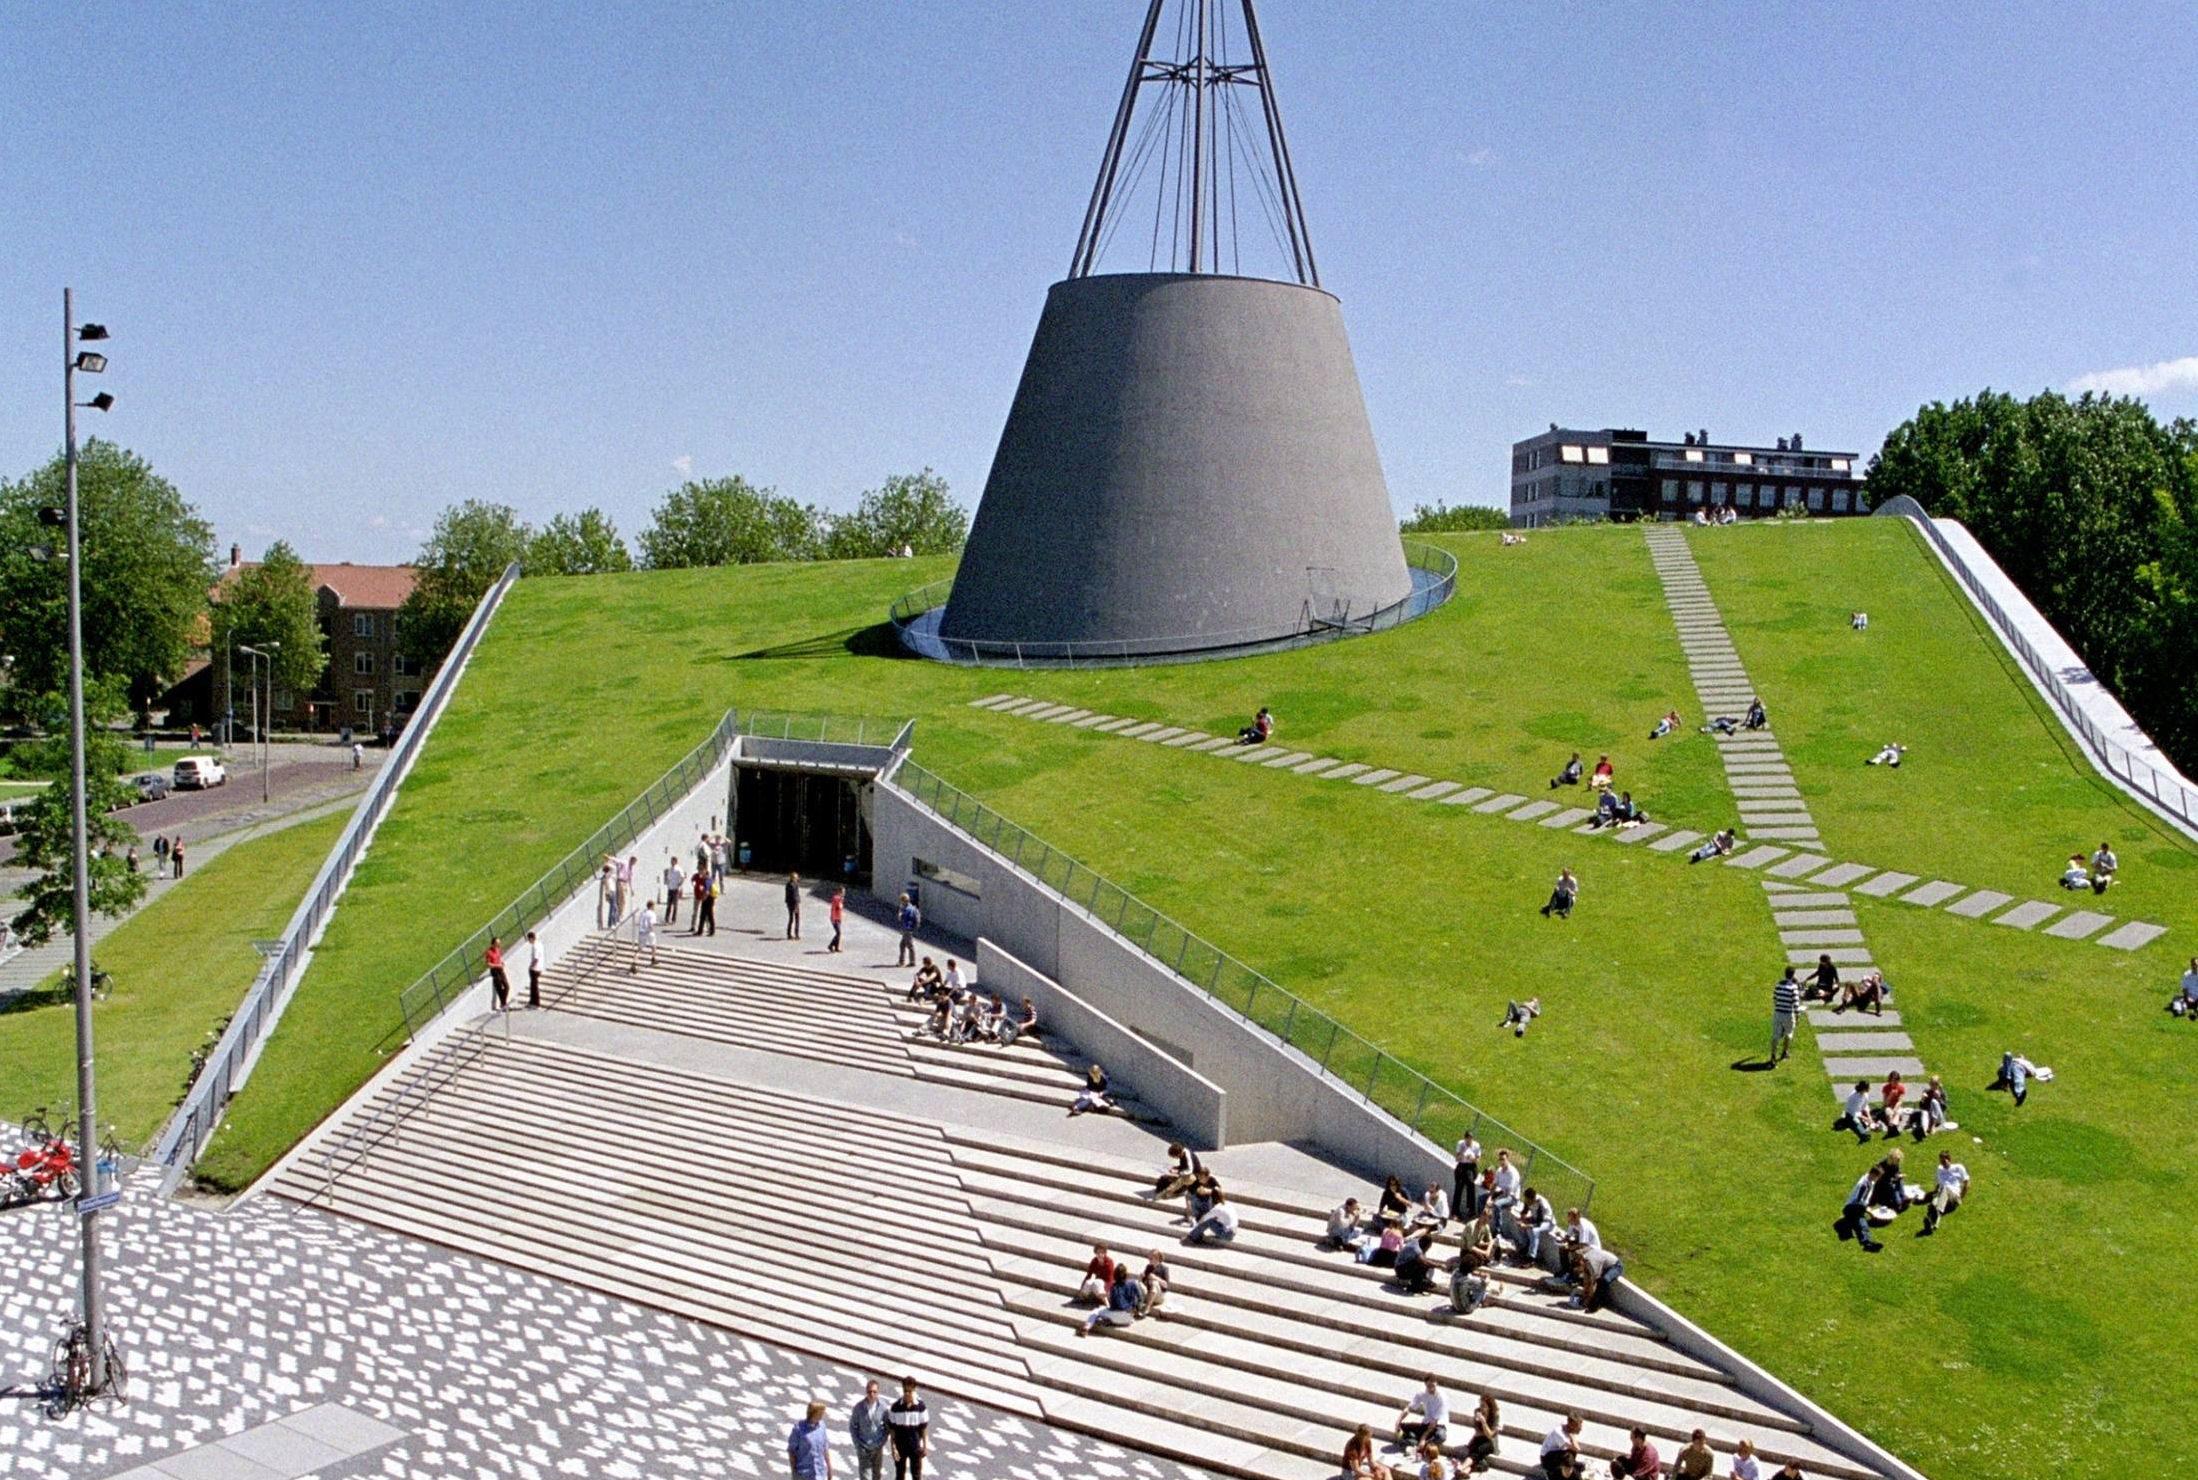
\includegraphics[height=8.65cm]{TUDelft/background-titlepage.jpg}};

            \fill [cyan!95!black!70!blue] (0,2.9) -- (0,5.35) -- (-.5,5.35) -- (-.5,2.9) -- cycle ;%squareNorthWest
            \draw [fill=black] (0,0) -- (11,0) -- (11,2.9) -- (0,2.9) -- cycle ;
            \fill [fill=cyan!65!blue!80] (7,-3.9) -- (12.4,-3.9) -- (12.4,-3.65) -- (7,-3.65) -- cycle;
            \node [shift={(0.8cm,-2.9cm)},textlabel,right]  at (current page.north west) {\textbf{\large{\textrm{\titel}}}};
            \node [shift={(0.8cm,-3.5cm)},textlabel,cyan!95!black!70!blue,right]  at (current page.north west)
            {\textbf{\large{\textrm{\subkop}}}};
            \node [shift={(0.8cm,-4.6cm)},textlabel,right]  at (current page.north west)
            {\normalsize{\naam}};
        \end{tikzpicture}};
    \end{tikzpicture}
\end{frame}
%==============================================================

\begin{frame}\frametitle{\textbf{\LARGE{\textrm{Introduction}}}}
	\begin{itemize}
		\item Literature survey.
		\item 21 papers on Multi-Tenancy.
		\item Published between 2006 - now.
	\end{itemize}
	\begin{figure}[H]
		\centering
		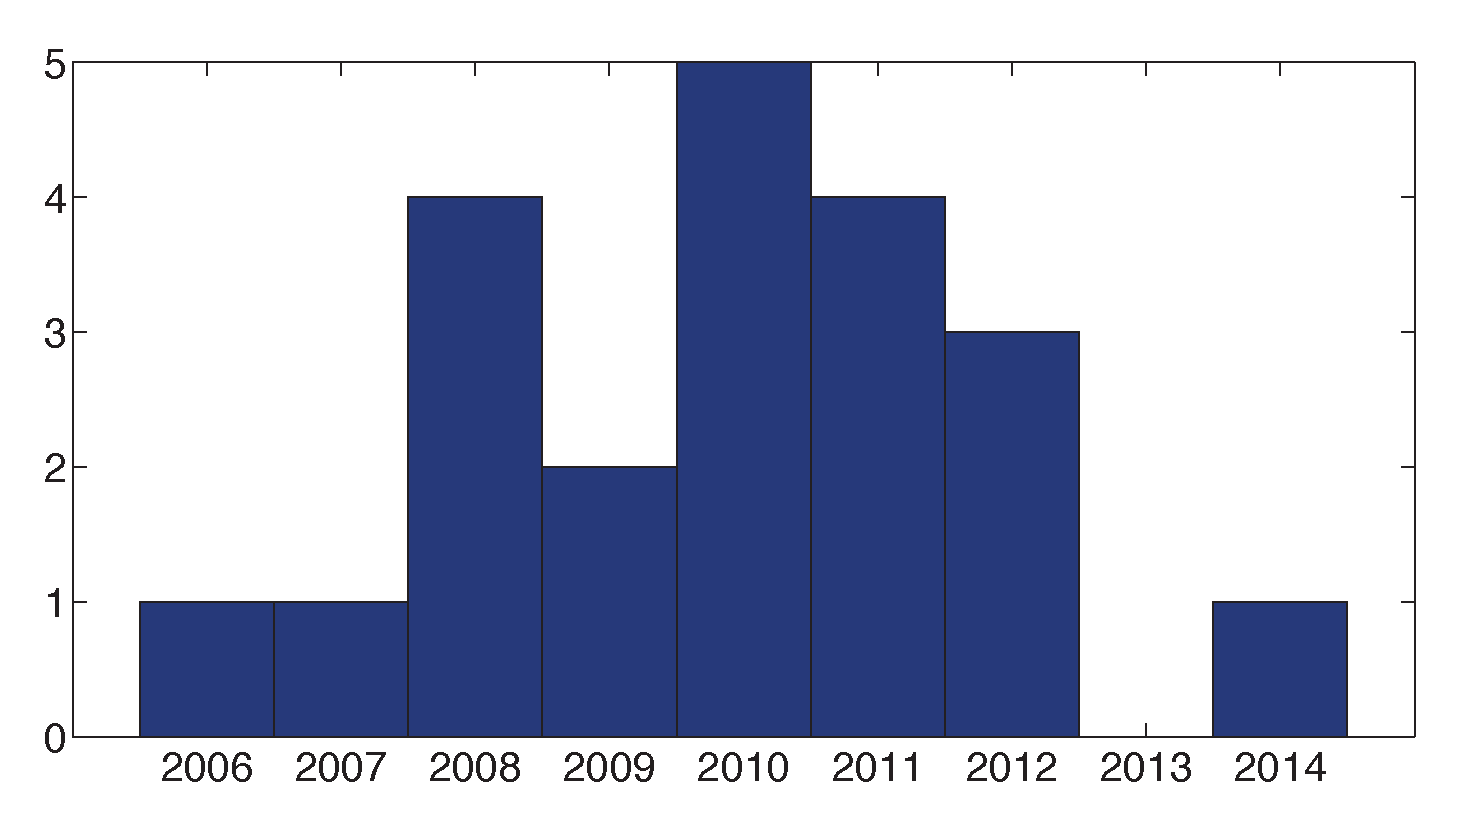
\includegraphics[width=.7\columnwidth]{../assets/papers.pdf}
		\caption{Referenced papers per year.}
	\end{figure}
	%Uitleg wat we gedaan hebben; Survey met als doel..
	%Indeling presentatie
	%Evt.: Uitleg dat we MT specifieke problemen pakken. (DB Schalen niet persé moeilijk, MT DB wel.., dat idee).
\end{frame}

\begin{frame}\frametitle{\textbf{\LARGE{\textrm{What is Multi-Tenancy.}}}}
	\begin{columns}
		\column{.7\textwidth}
		\begin{itemize}
			\item No official definition!
			\item Tenant: Group of users sharing view on app.
			\item Multiple tenants on the same instance.
			\item Key subjects:
				\begin{itemize}
				\item Security
				\item Scalability \& QoS
				\item Variability
				\end{itemize}
		\end{itemize}
		\column{.3\textwidth}
		
\includegraphics[width=.8\columnwidth]{images/large_questionmark.jpg}
	\end{columns}
\end{frame}

\begin{frame}\frametitle{\textbf{\LARGE{\textrm{The State of Security}}}}
	%TODO
\end{frame}

%TODO: Plaatje
\begin{frame}\frametitle{\textbf{\LARGE{\textrm{The State of Scalability}}}}
	\begin{itemize}
		\item Multi-Tenant applications must be scalable.
		\item Subjects in the application layer:
			\begin{itemize}
				\item Estimating resource usage per tenant, per user.
				\item Tenant placement \& resource allocation.
			\end{itemize}
		\item Subjects in the data layer:
			\begin{itemize}
				\item Scalable handling of extensible schemas.
			\end{itemize}
	\end{itemize}
\end{frame}

%TODO: Plaatje
\begin{frame}\frametitle{\textbf{\LARGE{\textrm{The State of Quality of Service}}}}
	\begin{itemize}
		\item Tenants should not be able to affect other tenants.
		\item Performance requirements may differ per tenant.
		\item Subjects:
			\begin{itemize}
				\item Aggressive tenant handling.
				\item Performance isolation.
			\end{itemize}
	\end{itemize}
\end{frame}

\begin{frame}\frametitle{\textbf{\LARGE{\textrm{The State of Variability}}}}
\end{frame}

\begin{frame}\frametitle{\textbf{\LARGE{\textrm{Research Opportunities}}}}
\end{frame}

\begin{frame}\frametitle{\textbf{\LARGE{\textrm{Research Opportunities cont'd}}}}
\end{frame}

\begin{frame}\frametitle{\textbf{\LARGE{\textrm{Questions and Discussion}}}}
\end{frame}


\end{document} 
